\section{Methods}
This section will be an examination of the experiments that will be performed to answer 
the research questions, as well as the implementation to do so. First, the software that was 
used to build the foundation for the RL framework will be discussed. Next, the implementation 
of the RL framework will be explained. Furthermore, the metrics and the experiments 
will be explained. 

\subsection{Architecture}
Each part of the architecture that will be used for the training and testing of 
the agent will 
be addressed. An overview can be seen in Figure \ref{architectureoverview}. \newline

\begin{Figure}
    \centering
    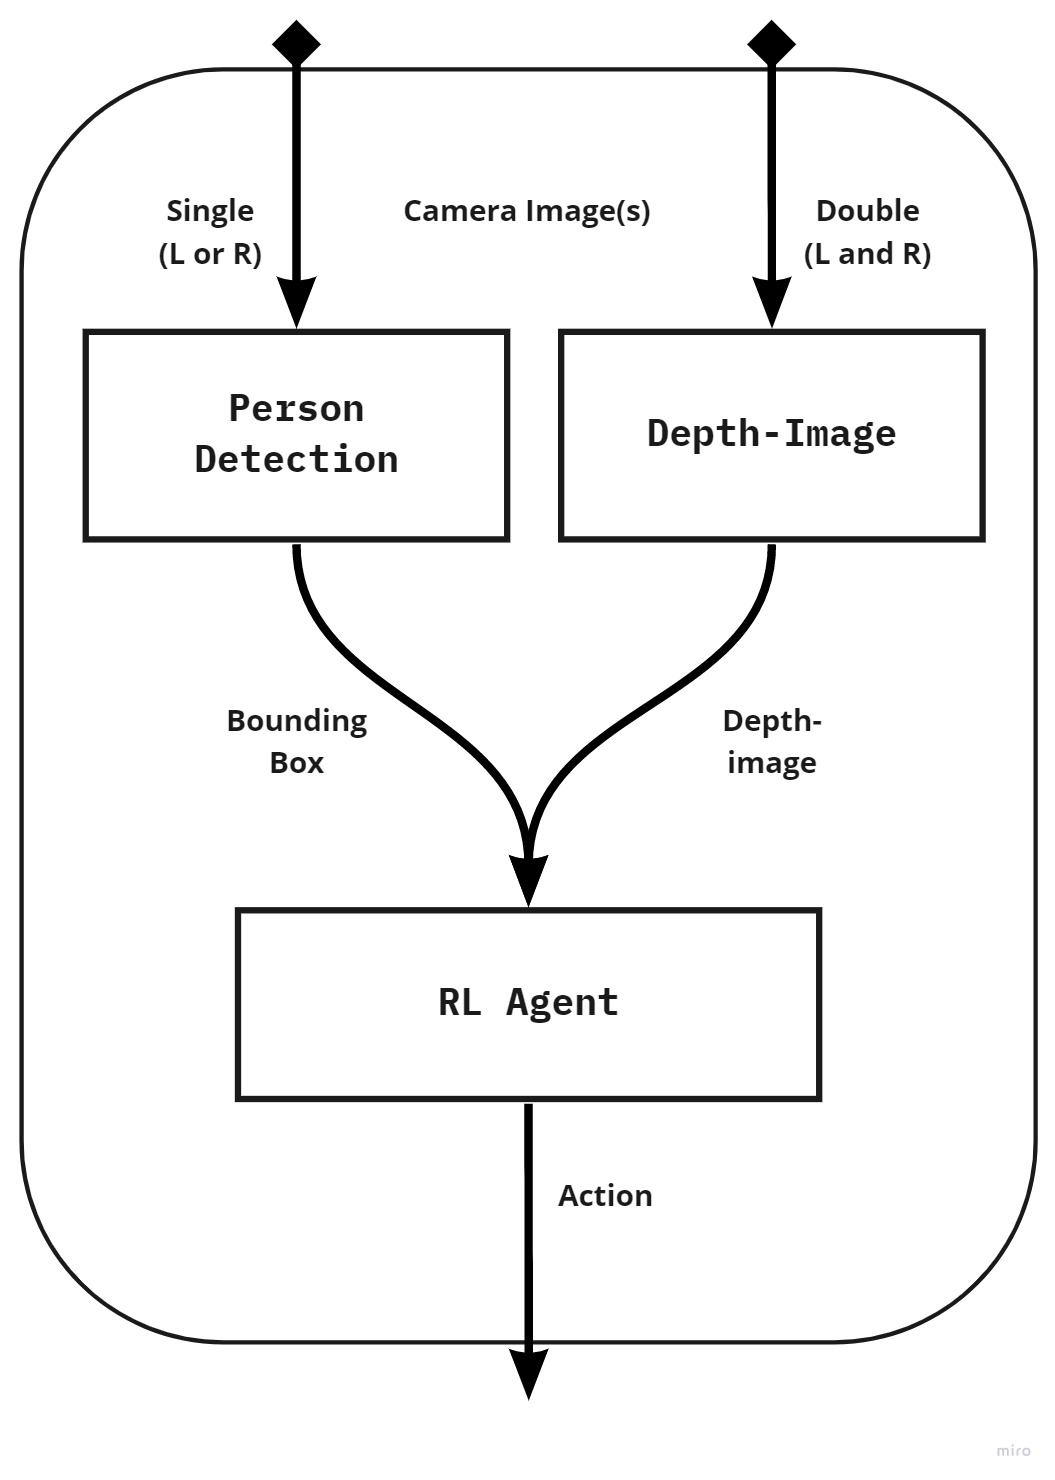
\includegraphics[width=\linewidth]{methods/Pipeline.jpg}
    \captionof{figure}{Overview of each element in the architecture used to perform 
    the experiments in}
    \label{architectureoverview}
\end{Figure}

\subsubsection{Simulation}
The most important aspect of the framework and architecture is the simulation system 
in which the drone will operate. As seen in Figure \ref{architectureoverview}, the 
simulation is the most crucial aspect in which the RL framework operates. The 
simulation is a combination of multiple aspects that will be discussed further, namely 
the person, AirSim and the physics engine defining the physical environment of the drone. 
Each aspect of the simulation environment will be discussed in the coming sections. \newline 

\noindent
\textbf{AirSim} \newline
The program that will be used to take control of a drone will be Microsoft's  
AirSim \cite{airsim}. AirSim is a coding library that is used in order 
communicate with drones instantiated in simulation environments or physical drones. 
Next 
to this, the program allows the user to instantiate a quadcopter directly in a 
virtual environment, together with simulated vision possibilities including a 
normal camera and depth-view. These views can be observed at the bottom of 
Figure \ref{airsim}.Furthermore, using the Unreal Engine \cite{unrealengine}, 
this program allows for a multitude of created environments to be used. This feature 
allows the ability to create or use different environments that systematically introduce 
variables to be tested.  What is more, AirSim has the ability to 
command the vehicles through a Python or C++ script, which makes AirSim very suitable 
to perform Deep Learning. What makes it even more attractive, is that AirSim allows 
easy connectivity with the PixHaw API, which makes it easy 
for the drone to be implemented on an actual physical drone in order to allow 
development for real-life applications. \newline

\begin{Figure}
    \centering
    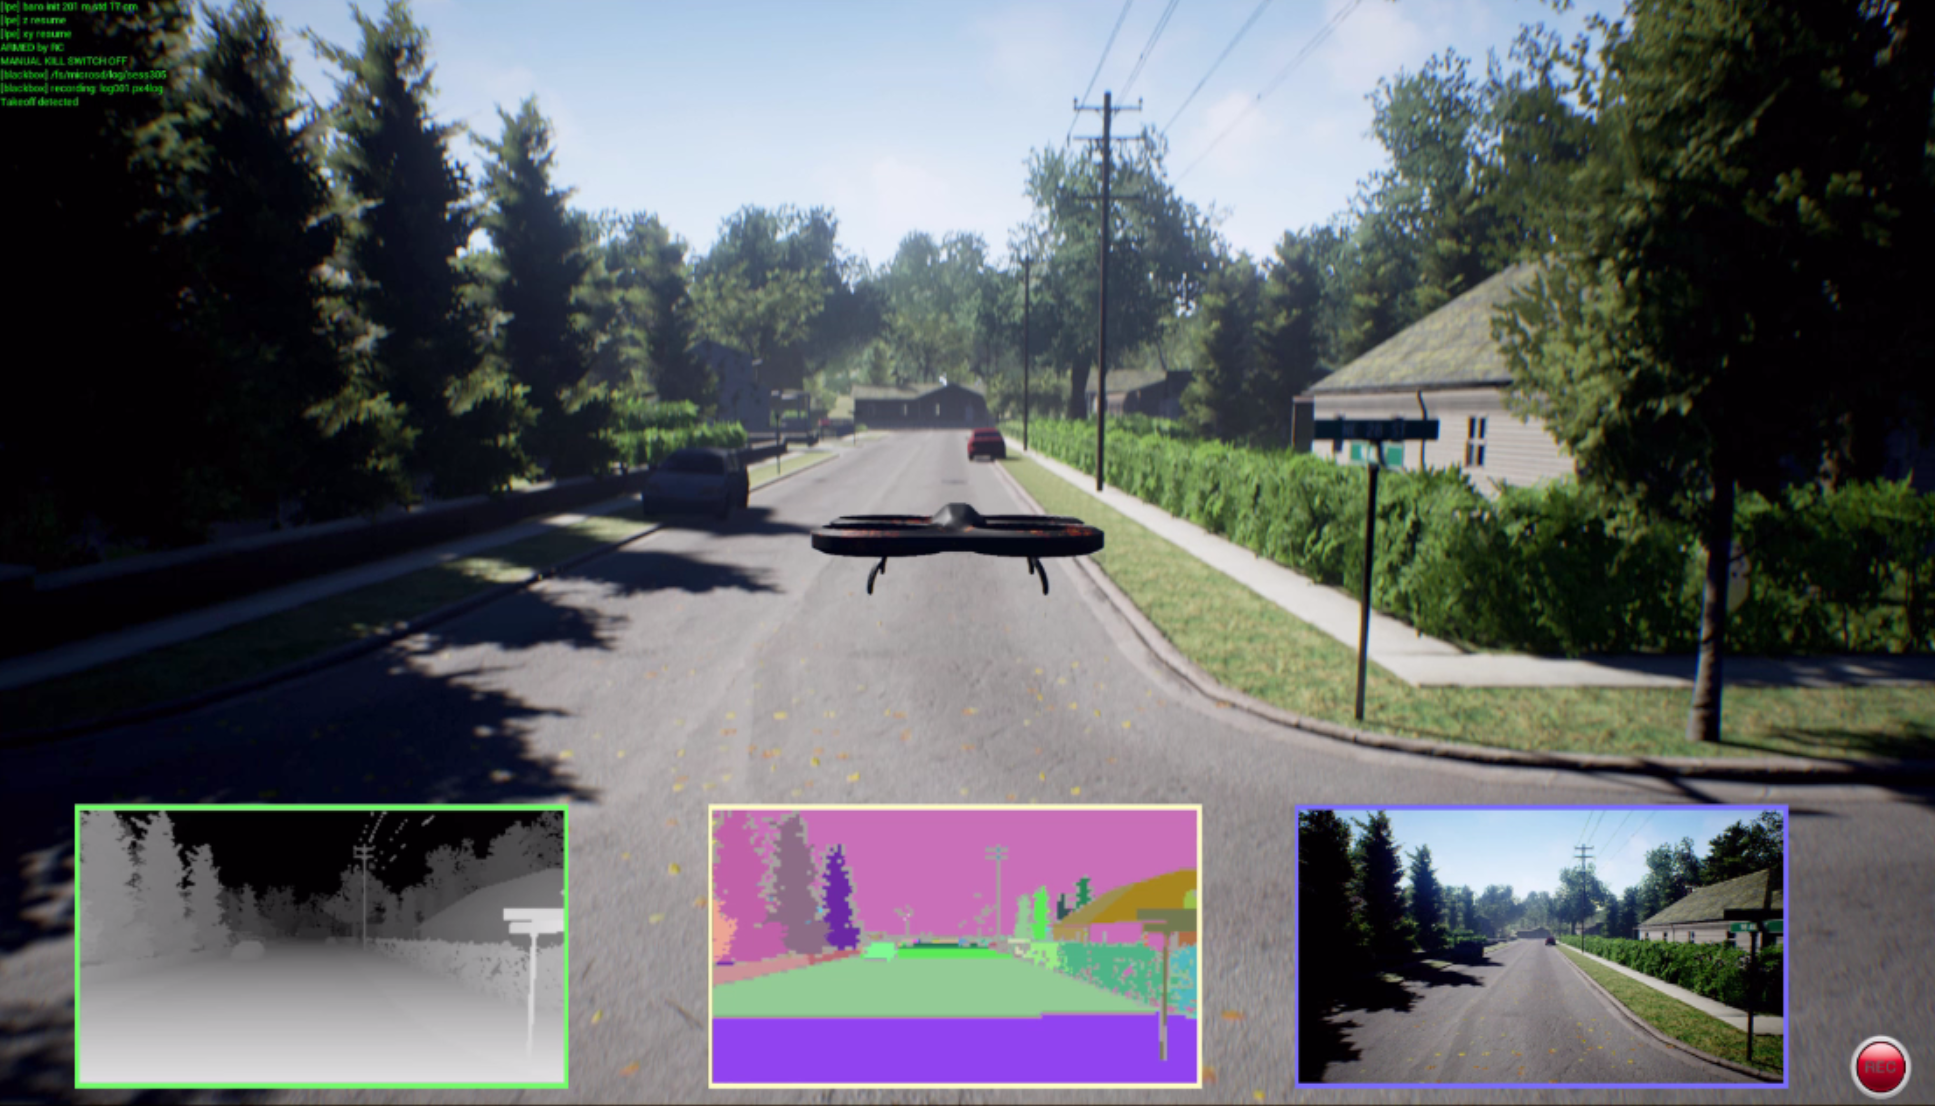
\includegraphics[width=0.8\linewidth]{methods/airsim.png}
    \captionof{figure}{The AirSim program features}
    \label{airsim}
\end{Figure} 


\noindent
\textbf{Environments} \newline
Another aspect of the simulation, is the physical environment in which the drone 
will fly. For this, three environments have been created. A set of agents will 
be trained and tested in each environment which will be specified in Section \ref{experiments}.
Snapshots of the environments from the top view are visible in Figure \ref{routes}.

\begin{Figure}
    \centering
    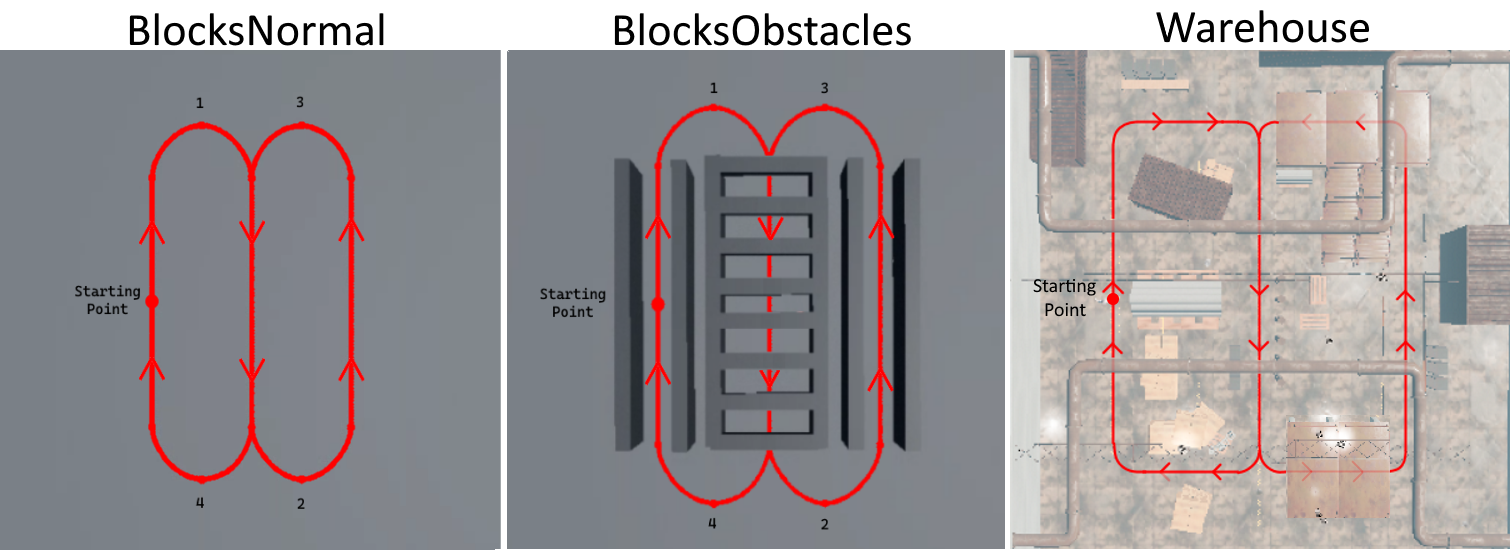
\includegraphics[width=\linewidth]{methods/WalkingRoutes.png}
    \captionof{figure}{The layout and obstacles for each individual environment and the 
    walking path of the person}
    \label{routes}
\end{Figure} 

The shape of the person's walking path inside of the environments are kept a steady 
variable. This shape was picked as a means of balancing the amount of time the person 
will be walking straight and making turns. At the same time, in order to keep an even amount of 
right and left turns, the need to have two left and right turns was kept in mind. For the 
Warehouse environment, a variation 
was used, where the turns of the person were expanded. 
Keeping the walking routes the same eliminates this variable as a possible explanation 
for why certain models might perform less well in certain tests. 

The people that the drone will be following can vary per environment. As will become clear 
in Section \ref{inputs}, the input states will not contain any information about 
the specific individual that is being followed. For this reason, during training time and 
testing time, a different target person can be implemented. Nonetheless, at any point in 
time there will be at most one person in the environment, which will be the person that 
the drone will have to follow. Again, in order to isolate the required task of the 
agent to follow an individual person, the choice has been made to not include multiple 
people. 

Looking at the implemented environments, the first environment will be BlocksNormal, which will 
consist of no obstacles for the 
agent to deal with. In this situation, the agent's ability to learn the follow-me behavior 
will be assessed. The second will be BlocksObstacles in which different types of 
obstacles have been added to simulate three different situations, namely: tight 
hallways, wide hallways and corners. Their locations can be seen in Figure \ref{areas}.
In this environment, the agents ability to deal with these situations will be gauged.
Finally, the Warehouse environments will contain similarly designed situations, 
however with much more details. Here, the objects consist of different types of 
objects and textures but create similar obstacles for the drone to avoid as in the 
BlocksObstacle environment. In this way, the behavior can be analyzed specifically by 
looking at how the agent deals with each specific situation to see whether the agents 
are able to generalize their behavior to new situations.


\begin{SCfigure}
    \centering
    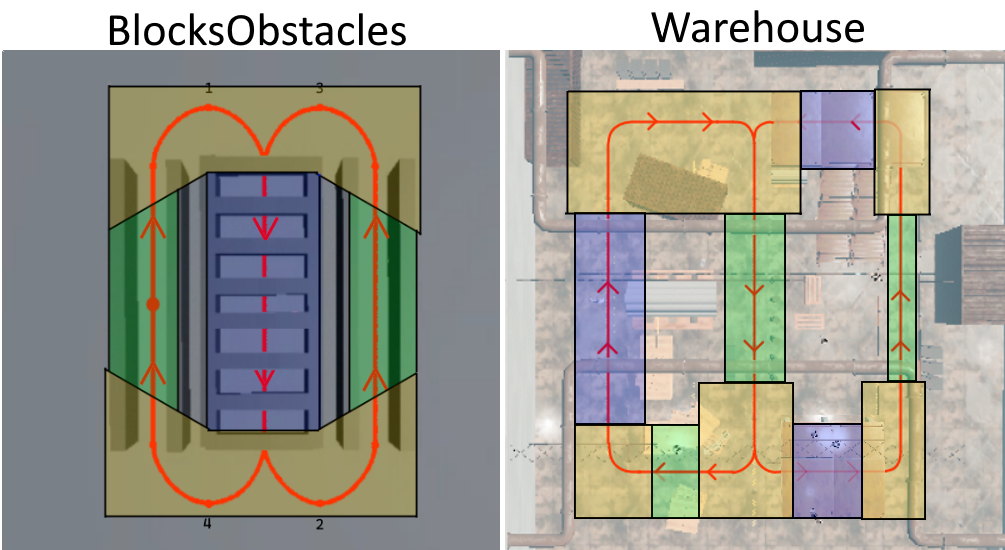
\includegraphics[width=0.66\linewidth]{methods/situations.png}
    \captionof{figure}[Locations of each type of situation in the environments]{Locations of each type of situation in the environments\newline\newline
    The areas correspond to the following situations: \newline
    Green = Tight hallways\newline
    Blue = Wide hallways \newline
    Yellow = Corners\newline\newline}
    \label{areas}
\end{SCfigure}


\subsubsection{Agent Structure}
In this thesis, a DQN will be implemented as an agent that will perform $Q$-learning. 
The choice for this type of learning has been made because 
of the aforementioned reason that the DQN can easily be implemented to be tested in 
new domains. Furthermore, its inputs are easily changed as necessary for the experiments that 
will be run. Now the overall architecture of the agent, which is the decision making body 
that is actually in control of the drone, will be described. \newline

\noindent
\textbf{Inputs} \label{inputs} \newline
The camera inputs of the agents will have a resolution of 128 x 72. Next to this image, the 
bounding box of the person in the view of the drone will be derived. This will provide 
the drone with information about the location and distance of the person in its camera view.
The bounding box will be retrieved using AirSim's Segmentation maps. These maps provide the 
same image as the view from the camera of the vehicle, but instead each pixel represents what object
is in view. An example of one such segmentation maps can be seen in Figure \ref{segmentationmap}. 
The color in this segmentation map for the person is preemptively set during initialization of the 
entire program, and when the drone receives this frame, it searches for the pixels corresponding 
to this color. When this is available, simply taking the extremes 
on both axes will provide the agent with the bounding box of the person. The pixels in 
this bounding box 
area will then all receive a -1 value while the rest of the image will be processed according 
to what type of combination of state-representation is chosen. These images could be 
stacked, which would result in the repetition of this process three times. The image 
itself could also be a depth map, in which case no further processing is done. If the image 
is a normal RGB image, it is first grayscaled. Doing this removes the three channels 
in an RGB image while still maintaining all of the required information. Before passing this 
state to the agent for training and 
decision making, the image is normalized in order to stay within a range of 0 to 1. An important 
note here to make is that the range of the bounding box in the image will stay -1, making the 
possible values for each input to the agent range between -1 and 1. This normalized image is 
then used as an input for the agent to decide on what action to take. \newline

\begin{Figure}
    \centering
    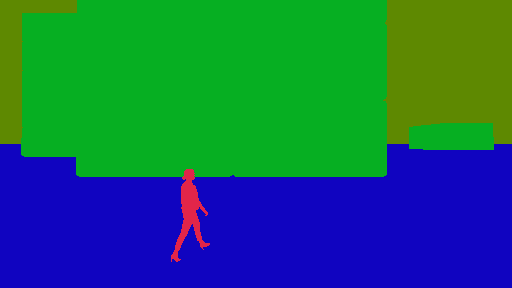
\includegraphics[width=0.7\linewidth]{methods/segmentation1616512266.6097646.png}
    \captionof{figure}{Segmentation Map from AirSim}
    \label{segmentationmap}
\end{Figure}

\noindent
\textbf{Network and Hyperparameters} \newline
Every type agent will be a variation of the DQN agent and will therefore, contain the same 
network. This network can be seen in Figure \ref{network} and the specific 
architecture details can be found in Table \ref{tab:NetworkArch}. Being quite modest 
in size, this neural network has approximately 2M parameters, 
which makes it computationally easy to train and deploy. 
This architecture has been chosen because of the fact that a convolutional network is required, as 
it is supposed to process image data. However, it does not require to be a large network as the 
limitation of this thesis is that it should stay resource efficient. Furthermore, it is only required 
to make decisions upon these images, so the network architecture does not necessitate a network 
that is extremely large. The optimizer that will be used is Root Mean Square Propagation 
(RMSProp) \cite{rmsprop} with a learning rate of $0.001$. \newline

\begin{table}[h]
    \centering
    \caption{Network Architecture of the DQN}
    \label{tab:NetworkArch}
    \begin{tabular}{l|c}
    \multicolumn{1}{c|}{\textbf{Layer}} & \textbf{Parameters}                                \\ \hline
    Convolutional layer                 & 32 Filters of 8x8 and stride 4                     \\
    Convolutional layer                 & 64 filters of 4x4 and stride 2                     \\
    Convolutional layer                 & \multicolumn{1}{l}{64 filters of 3x3 and stride 1} \\
    Fully connected layer               & 512                                                \\
    Fully connected layer               & 128                                               
    \end{tabular}
\end{table}


\begin{Figure}
    \centering
    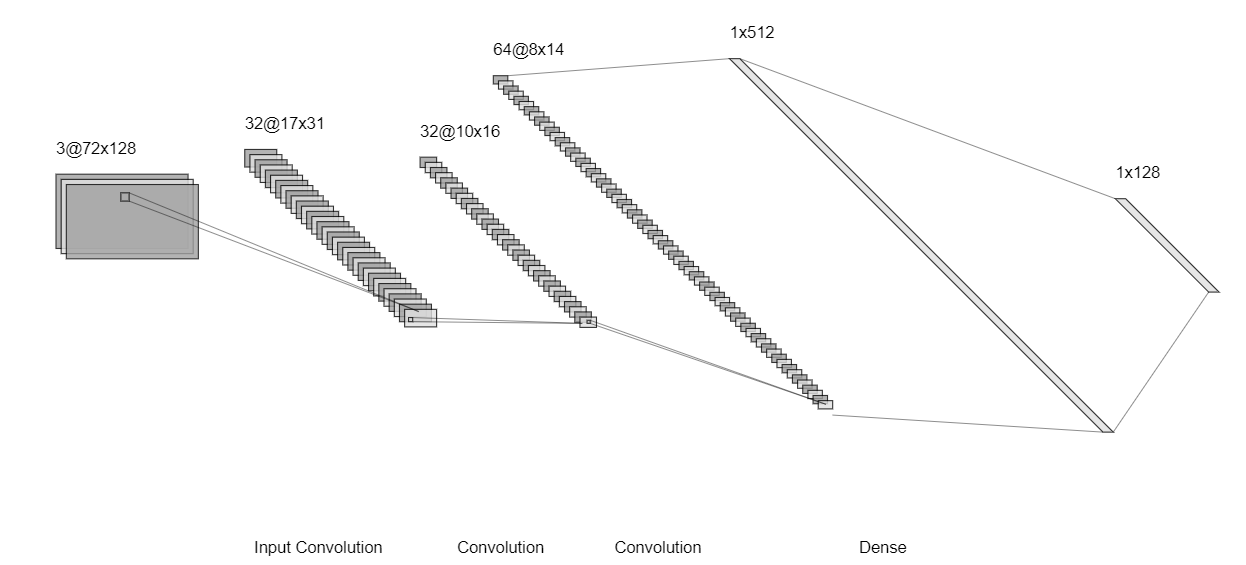
\includegraphics[width=\linewidth]{methods/network.png}
    \captionof{figure}{Network Architecture}
    \label{network}
\end{Figure}

\noindent
\textbf{Outputs} \newline
The DQN's output will be an integer
between the range of 0 and 5, each of these representing an action as is illustrated in 
Table \ref{fig:actions}. These actions have been chosen so that the agent is able to 
manoeuver in the environment in most directions. The ability to orient itself 
is a requirement in order to change its direction. However, this orientation is only 
possible on a horizontal axis. Vertically, the drone will remain at a static height. Its 
vertical orientation is unable to change as these movements would also result in a horizontal 
displacement. Changing the camera positions is synonymous with moving the drone itself. 
An important note to make is that the drone is unable to move backwards. The reason for 
this lack of movement is because the drone is unable to sense what is happening in the 
back. Nonetheless, the movements to the right and left have been included because the drone 
is able to partially observe the obstacles in these settings. 

\begin{table}[h]
    \caption{Mapping from network output to actions}
    \label{fig:actions}
    \centering
    \begin{tabular}{ll}
    \textbf{Integer} & \textbf{Action} \\
    0                & Do nothing      \\
    1                & Orient right    \\
    2                & Orient left     \\
    3                & Go straight     \\
    4                & Move right      \\
    5                & Move left      
    \end{tabular}
\end{table}

\subsubsection{Agents and variations}
In order to answer the research questions (\ref{RQs}), a variation of the DQN will 
be implemented. There will be two types of agents and an additional of two variations that 
will be used in this dissertation. Each of these variations will be introduced and discussed 
here. \newline

\noindent
\textbf{Baseline} \label{baseline} \newline 
First, a baseline that does not use RL techniques but more straight forward heuristics 
to decide on an action will be implemented. The method used for this, has been inspired by the 
techniques that are used in drone control when RL is not used, as discussed in Section 
\ref{baselineliterature}. These methods use the simple assumption that the drone is 
tracking the object when a set of conditions are met. These conditions include that the 
object is centered inside of the camera input and that the size of the object corresponds 
to a certain proportion. From these conditions the distance to the object can be derived 
and whether the drone is looking at it. 

Using these principles, the following agent has been developed. 
With the received camera input, the baseline agent determines where 
the bounding box is in the image. If the center of this bounding box is in the left side view, 
the agent will rotate left. If the bounding box is in the right side of the view, 
the agent will rotate right. If the bounding box center is within a range of the center 
of the view, the agent will check what the height of the bounding box is to see how much it 
differs from the goal height. The goal height being 20\% of the image height, an additional 
margin of error will be permitted in order to prevent constant movements of the agent. In the 
case that the bounding box height is within this margin of 25\%, 
the agent will not move. In the other case, the agent will move forward, coming closer to the 
person. 

Using these methods removes the 
need to perform calculations about the exact location of the person, while also maintaining 
sufficient distance from the person. At the same time, as will be elaborated upon in 
Section \ref{rewardfunction}, these values have been fine-tuned with the reward function in order 
to also maximize the reward function using this method. This agent does not require any training 
and is therefore simply used as a baseline model in order to compare the RL models to. \newline

\noindent
\textbf{State-representation variations} \label{stackedimages} \newline
The RL agent that will be used will be a DQN. However, its state can vary and these will 
be tested accordingly. In this thesis, two such variations will be implemented and investigated.

The first variation to the state-representation that can be made is the use of stacking.
Considering the limitations of this study to maintain a low computationally functioning agent, 
the decision has been made to opt for video input as a means to communicate directionality to the 
agent. The use of RNNs, would require too much computing power. This has been implemented 
by taking three consecutive frames from the environment with 0.1 second intervals
as a means to form a video. This video can also be considered a stacked image of the last three 
frames. This stacked image can be created by getting a frame from 
AirSim (either normal or depth), deriving from it the bounding box, 
processing it as described in Section \ref{inputs} and then finally, simply to stack 
them in a 3-dimensional image as can be seen in Figure \ref{pipeline}. This object is now used 
as the input for the agent.  

\begin{Figure}
    \centering
    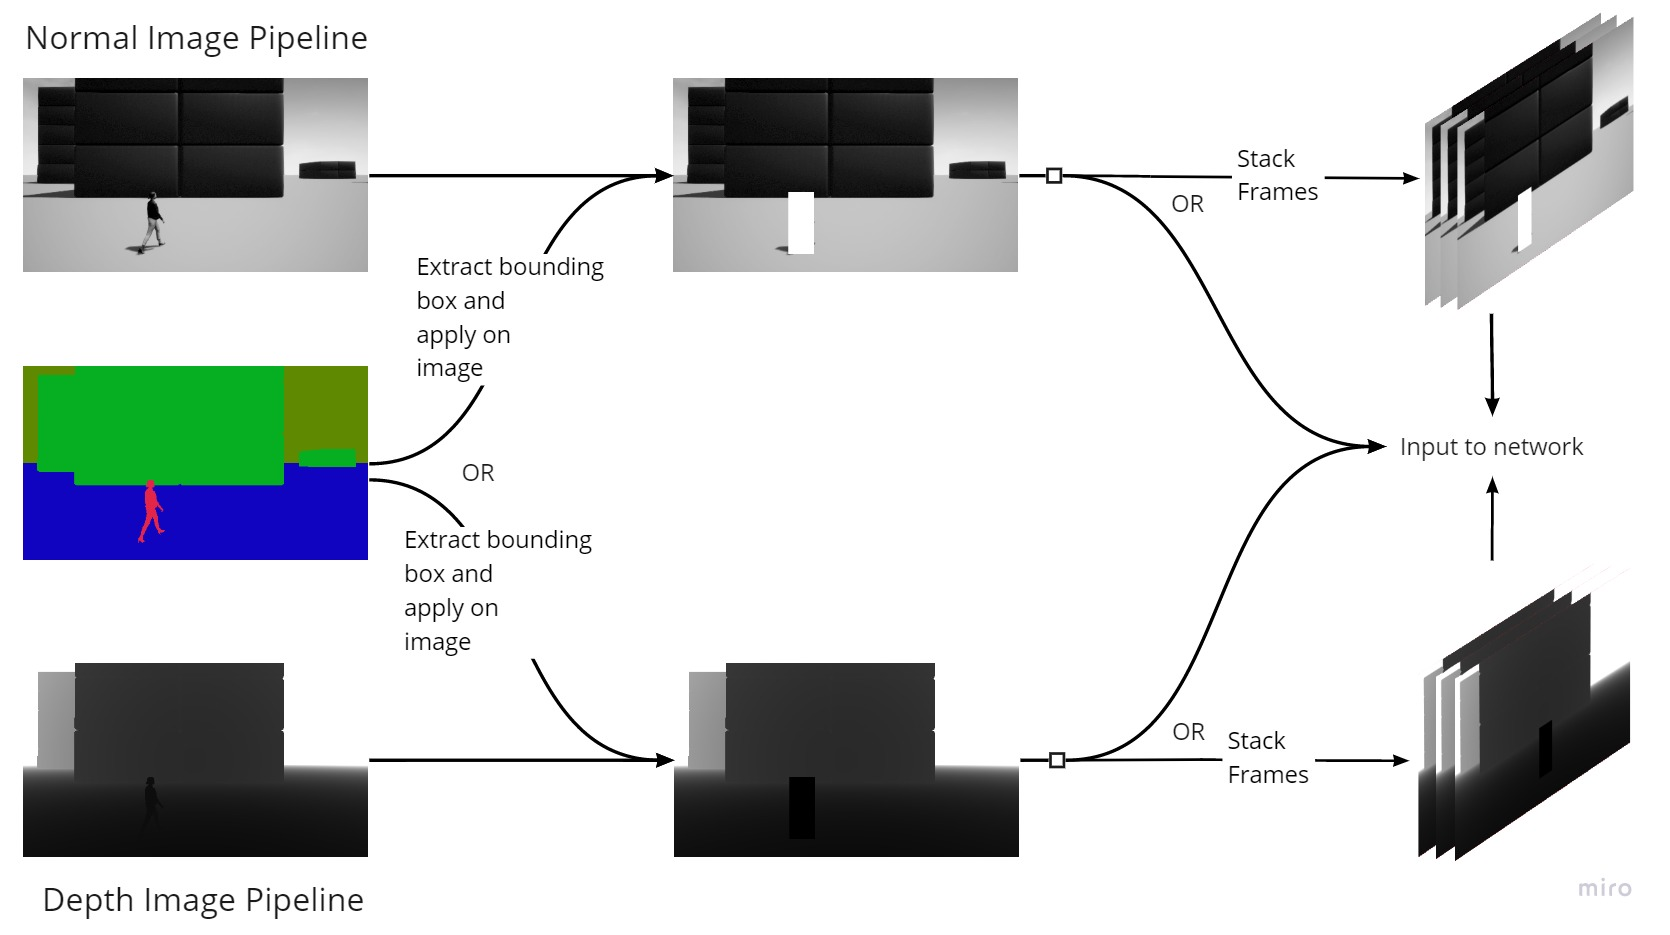
\includegraphics[width=\linewidth]{methods/StateProcessing.jpg}
    \captionof{figure}{Pipeline to process AirSim images in order to create a state for the 
    DQN agent}
    \label{pipeline}
\end{Figure}

Another variation is the use of depth images. 
In order to allow the agent to sense obstacles in its surroundings, the choice has been made 
to us depth maps. This option combines the ability for the agent to receive image input, 
perceive the person and detect the distances to the obstacles around it. AirSim provides 
the ease of simply requesting depth maps from the environment, giving the agent access to 
the ground truth distances to all of its surroundings. Important to note, these depth 
maps can easily be combined with the stacking of them, allowing for all of the possible 
combinations of these agents to be tested.  \newline

\subsubsection{RL Framework} \label{RLframe}
The reinforcement learning framework are also an important part of the implementation that 
require some discussion. The use of a python library that builds 
upon the machine learning library Tensorflow, called TF-Agents has been opted for. Tensorflow is, 
in itself, 
a library that abstracts machine learning algorithms to be implemented. Adding to this,  
TF-Agents allows for a high-level abstraction of the RL implementations. Nonetheless, 
more specific RL environment aspects require to be developed, each of which 
will be elaborated upon in the next sections. \newline

\noindent
\textbf{RL Environment} \newline  
An important aspect of reinforcement learning is the RL environment. Here we refer not to 
the simulated environment where the drone is flying in, but the RL environment that creates 
the states 
and returns rewards where necessary, as seen in Figure \ref{architectureoverview}. The agent 
interacts with the RL environment, which again interacts
with the simulated environment in order to get the required information. Crucially, RL algorithms 
tend to operate in episodes. An episode is characterized by a beginning state and a terminal state, with 
transitions of steps that the agent is taking in between. After this terminal state, the environment 
resets and a new episode begins. 

In this implementation, the starting state of the person is directly behind the person at a 
slight distance. Keeping this initial distance from the person removes a bias in reward in 
earlier states of an episode. After this, a step is taken by the agent. This step process 
is defined as follows. First, a state is retrieved, which is performed as described in Section \ref{inputs}. 
Consequently, an action is chosen by the agent according to this state after 
which a reward is calculated for this new state. Finally, in each step, an assessment will be made as 
to whether an episode has ended, to determine whether the terminal state has been reached. 
This will be done by checking whether one of the next three requirements have been met: the agent 
has collided with an object, the agent has no bounding box in its camera, meaning the person was 
lost from its view; more than 50 steps have been taken. These conditions ensure that an episode 
consist of a finite sequence of actions for the DQN to be able to learn from. Between these episodes, 
the environment resets. This reset makes sure that the drone is reinstantiated 
to the correct position. In this case, the drone is being positioned directly behind the person and 
made sure to be oriented towards the direction of the person as well. These resets are meant as means 
to not waste time in state-spaces during training time that are not conducive for the agent to learn. 
States where it has collided or loses sight of the person are not relevant for the drone in order to 
learn how to follow successfully. Therefore, before too much time has been lost in these states, the 
environment resets to a moment from where it can continue its learning process successfully. \newline

\noindent
\textbf{Training} \newline  
Before the models can start training, some preparatory steps are performed. DQN requires a replay 
buffer where it stores a large dataset of 
experiences. This is necessary for the DQN as it requires samples from this buffer as an input 
for the network for each training step. Since this would also cause the primary training steps to be 
skewed, it's necessary to fill part of the replay buffer before training begins. Therefore, before training 
is started, an agent that performs random actions moves about in the world for 500 steps, filling 
a portion of the replay buffer, which has a size of 10,000 experiences total. This makes sure that an initial portion of the state-space 
is explored already before training begins.  

Next, the training process can be described as a loop where the same steps are being taken each time, 
also referred to as an epoch. 
This loop starts by performing 50 movements in the environment. These 50 movements correspond to a full 
episode before the environment resets. Some of the earlier episodes might not reach their 50 steps 
limit, however, nevertheless, a total of 50 steps will be taken before the network is trained on 
these experiences. This stabilizes the increase in replay buffer size throughout each epoch. 
The batch size of a sample is 64 and each model will be trained either to convergence or 
2000 epochs. 

It is important to note that the TF-agents library maintains two policies for an agent. One
collect policy which is meant to always keep a degree of randomness in order to always keep some 
level of exploration. Next to this, is an evaluation policy which is the optimal policy the 
agent has learned. Every 50 iterations, an evaluation step is taken. Here, 10 episodes are 
being played by the evaluation policy. The required metrics, as discussed later, are stored and 
the training loop continues. \newline

\noindent
\textbf{Reward Function} \label{rewardfunction} \newline  
The most important aspect of RL is the reward function. Since learning in this context depends on the 
maximization of the reward function, the behavior that the agent will learn is highly dependent 
on this reward function. In this thesis, the choice has been made for an easily-developed sparse reward 
function. This is because, as mentioned before, there is no need to imbue the agent with pre-determined 
knowledge about how to reach the goals. This will allow the agent freedom in interpretation about 
how to solve this problem and not limit it to behavior decided upon by the developers. 

The reward function requires a connection from the state input. If this is missing, 
the agent is unable to actually perceive the impact of its actions on its states. To 
solve this problem, the bounding box will be used as an object to determine the reward, 
considering as it contains both information about the relative location as well as the distance 
to the person. Here, similar assumptions as the baseline will be made about relative location of 
the person, as well as its distance. The person should simply be in front of the drone, where 
centering the person in the middle of its camera view is included in the reward function. 
With regards to the distance to the person, a goal bounding box height has been determined 
using the distance to the drone. The goal distance to the person has been determined to be 
four meters, which, combined with the height of the drone, results in the person 
taking up 30\% of the image height. Combining both the centering and the distance 
conditions in a reward function results in the following set of rules. 
 
If there is a 
bounding box and no collision is happening, there are three conditions that are required to be met.
The first of these is the location of the $x$ value of the bounding box center. When this value 
is within a 20\% range of the center of the image, this condition is met. The second condition to be 
met is that the height of the bounding box is within a 30\% range of the goal height.
The final condition to be met is that the location of the 
$y$ value of the bounding box center should fall in the top 80\% portion of the image. This ensure 
that the drone is not positioned too close to the person. 
When all of these conditions are met, the reward is determined to be 1. In case of detected collision 
or a bounding box is missing, a -1 is returned. All other cases return a 0. 

In all of the tests, the reward function is kept a constant, in order to use this 
function as a metric for the performance of each agent. This way, all of the 
tests can be compared measured according to the reward received. \newline

\noindent
\textbf{Metrics and Methods of Analysis} \label{metrics} \newline  
The metrics to evaluate the training process, the follow-me performance and the behavior will be discussed.
Multiple perspectives will be taken. First, the training process is evaluated according 
to certain metrics. Next, overall performance metrics will be used as well. Finally, in order 
to compare the behavior of each agent, some formalizations will be introduced. 

An overall crucial metric, which will be used throughout this thesis, is the average 
return. In this metric the average reward that was gathered in an episode is recorded. 
This metric will be used to evaluate both the training procedure but also the agent's overall 
performance. As this metric encapsulates all of the requirements of the agents behavior, namely 
obstacle avoidance, person centering and keeping its distance. 

Metrics specific to the training procedures are the following. First, next to the average return, 
the average length of an episode
will be tracked. Since the 
episode can end early when a crash happens, or the person is out of sight, the longer an episode 
takes, the better the drone is at following the person. The cap here is at 50 steps, 
since that is when an episodes resets regardless. During the evaluation step there is a variation 
to these metrics. Instead of the average episode 
length and the loss, the minimum and maximum return are being recorded. These express the worst 
episode and the best episode that the model performed. The preferred situation is where the range 
between these two value is not too large. However, if that is not the case, looking at these 
extremes can shed a light on where the model is still lacking. 

With regards to quantifying the agent's behavior, a number of analysis techniques have been used 
to get in-depth information. First, for each of the 50 possible 
time-steps that an episode can last, the average received reward will be recorded. This 
information gives insight into how an average episode progresses for the agents and 
express potential bottlenecks of the agent as it showcases what the distribution is of the 
received reward through an average episode. Next to this, the paths the drone has taken 
throughout the test run and the location and type of episode ending will also be recording. 
This information provides data about the behavior of the agent and in which situations 
it is struggling the most. All of these aspects will be used to draw conclusions 
about the performance and behavior of each individual agent. 


\subsection{Experiments} \label{experiments}
In order to answer the research questions from this thesis a set of experiments will be run 
in the effort to answer them. The experiments will be performed per environment, each of them 
increasing in complexity. First, tests will be run in BlocksNormal, after which BlocksObstacles 
will be used to run tests in. Finally, tests will be run in the Warehouse. These tests together with 
the research question they answer, are illustrated 
in Figure \ref{im:experiments}. Each will be discussed in the following sections. 

\subsubsection{BlocksNormal}
First, four agents will be trained and tested in the BlocksNormal environment. The procedure 
in which this will happen, will interchange training with test sessions. Primarily, a DQN 
with single normal images and a DQN with stacked normal images will be trained. After this, 
both of them will be tested. The best working state-representation will be used for the final 
agent to be trained using depth images. This means that either a single depth or a stacked 
depth image DQN will be trained and tested. Finally, a baseline will also be tested and used 
for a comparison. After all of these tests have been run, the behaviors will be analyzed together 
with their overall performance. This means that each of the agents will be compared to the baseline 
in order to quantify how much better the RL agents perform compared to the baseline. 

\subsubsection{BlocksObstacles}
The second procedure will be performed in the BlocksObstacles environment and this 
will be performed in the exact same order as the previous environment. However, in the end, 
the performance will not simply be compared to the baseline. After the two tests in the 
BlocksNormal and the BlocksObstacle environments, the expectation is that there is a 
degradation in performance. This proportion of degradation will be used to compare the 
decrease in performance of each RL agent as well. Performing this comparison will give insight 
in whether the agents are comparatively better at handling this environment than the baseline. 
Finally, the best working agent in this environment will be retrained using a slightly modified 
reward function. This reward function will have tighter margins. Where the normal reward function 
had a margin of 25 \%, this one will be performed using 10 \%. Performing this test will 
reveal how the behavior can be targeted using the reward function. 

\subsubsection{Warehouse}
Finally, training and tests will be performed in the Warehouse environment. Starting by 
testing and comparing both the best working RL agent from the BlocksNormal and BlocksObstacles 
environment. The better working model of these will be retrained inside of the Warehouse environment. 
Performing these tests will give insights in to how much each agent was able to transfer knowledge from 
its trained environment to this new environments. Comparing these models to the baseline degradation, 
similarly to the previous environments, will again show how much better the RL agents are. 

\begin{Figure}
    \centering
    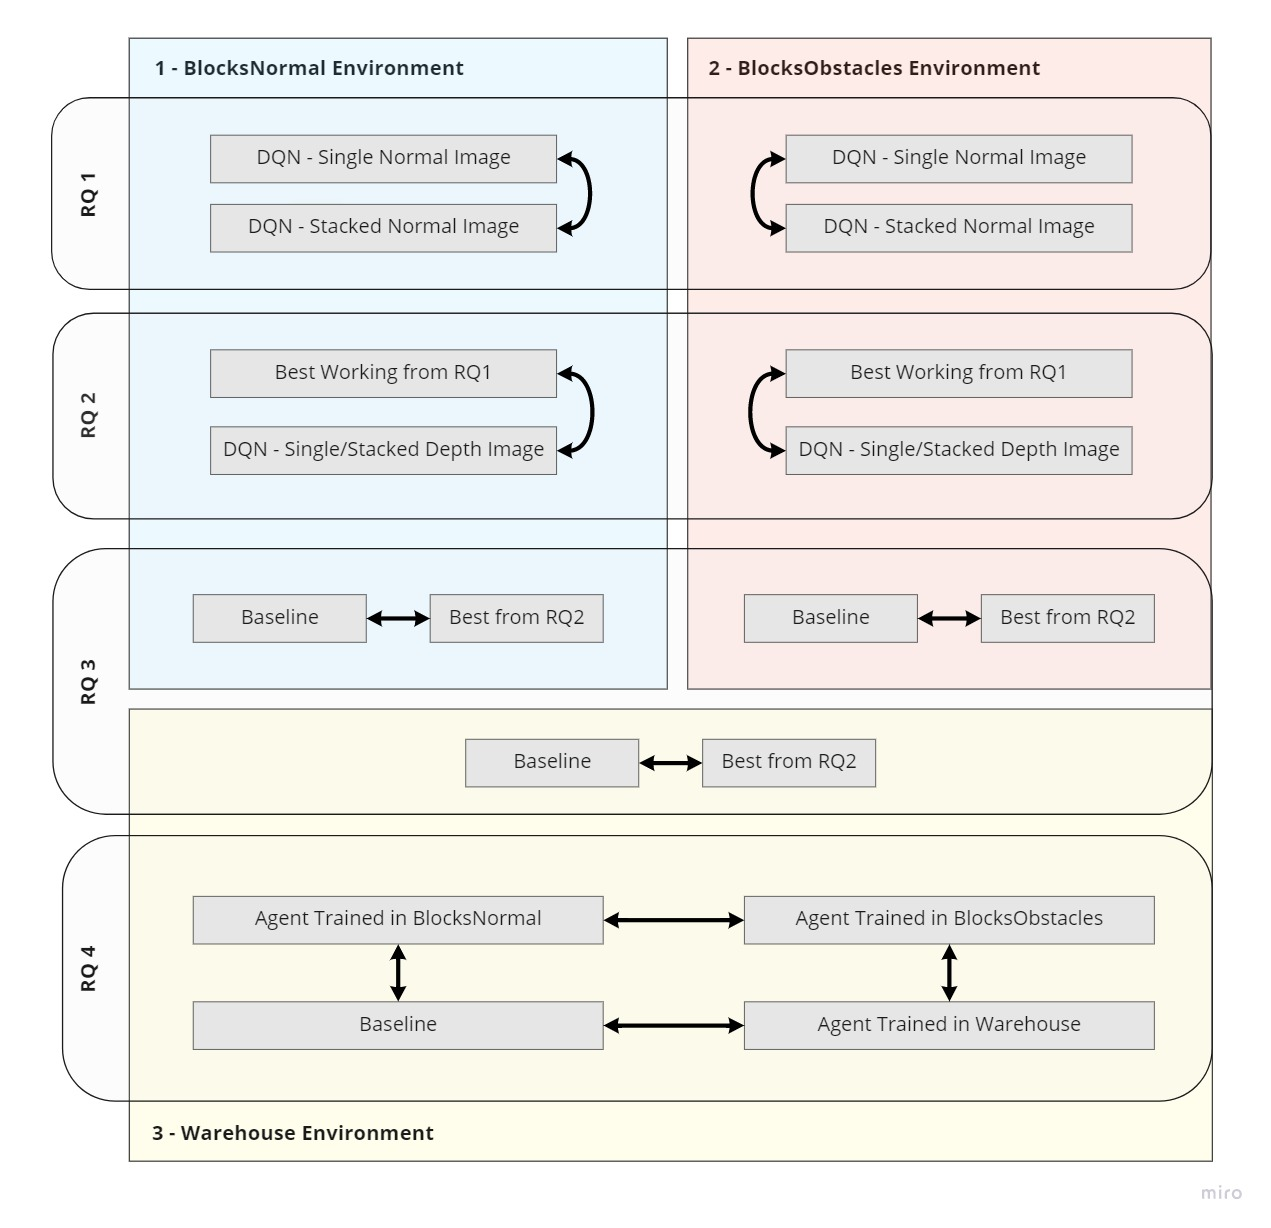
\includegraphics[width=\linewidth]{methods/experiments.jpg}
    \captionof{figure}{Experimental procedure that will be followed. The order will be to start 
    with the BlocksNormal environment, moving to the BlocksObstacles and ending with the Warehouse}
    \label{im:experiments}
\end{Figure}
